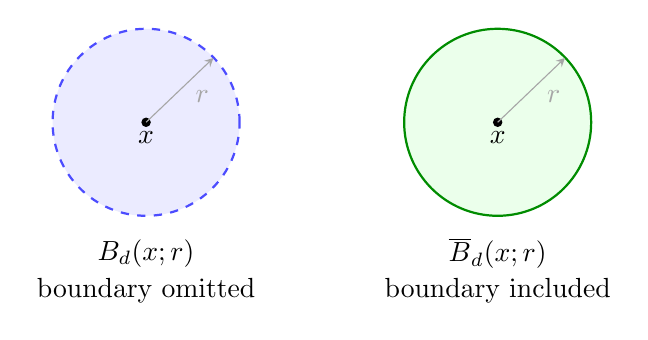
\begin{tikzpicture}[scale=0.95,>=stealth]
  \fill[blue!8] (0,0) circle (1.25);
  \draw[blue!70,thick,dashed] (0,0) circle (1.25);
  \fill[black] (0,0) circle (1.8pt);
  \node[below] at (0,0) {\(x\)};
  \draw[->,gray!70] (0,0) -- (0.9,0.86);
  \node[gray!70] at (0.75,0.35) {\(r\)};
  \node at (0,-1.75) {\(B_d(x;r)\)};
  \node[align=center] at (0,-2.25) {boundary omitted};

  \begin{scope}[xshift=4.7cm]
    \fill[green!8] (0,0) circle (1.25);
    \draw[green!55!black,thick] (0,0) circle (1.25);
    \fill[black] (0,0) circle (1.8pt);
    \node[below] at (0,0) {\(x\)};
    \draw[->,gray!70] (0,0) -- (0.9,0.86);
    \node[gray!70] at (0.75,0.35) {\(r\)};
    \node at (0,-1.75) {\(\overline{B}_d(x;r)\)};
    \node[align=center] at (0,-2.25) {boundary included};
  \end{scope}
\end{tikzpicture}
